% This is samplepaper.tex, a sample chapter demonstrating the
% LLNCS macro package for Springer Computer Science proceedings;
% Version 2.21 of 2022/01/12
%
\documentclass[runningheads]{llncs}
%
\usepackage[T1]{fontenc}
% T1 fonts will be used to generate the final print and online PDFs,
% so please use T1 fonts in your manuscript whenever possible.
% Other font encondings may result in incorrect characters.
%
\usepackage{graphicx}
% Used for displaying a sample figure. If possible, figure files should
% be included in EPS format.
%
% If you use the hyperref package, please uncomment the following two lines
% to display URLs in blue roman font according to Springer's eBook style:
\usepackage{hyperref}
\usepackage{color}
\renewcommand\UrlFont{\color{blue}\rmfamily}
\urlstyle{rm}
%
\usepackage{caption}
\usepackage{subcaption}
\usepackage[htt]{hyphenat}
\usepackage{amsmath}
\usepackage{amssymb}
\usepackage{booktabs}
\usepackage{multirow}
\usepackage{array}

\begin{document}
%
\title{Video-Text Multi-Instance Retrieval in Egocentric Video: From a JPoSE Baseline to AVION ViT-L Fine-Tuned with Symmetric Multi-Similarity Loss on EPIC-KITCHENS-100}
%
\titlerunning{Video-Text Multi-Instance Retrieval on EPIC-KITCHENS-100}
%
\author{ Nicolás Rozo Fajardo\inst{1} \and
Santiago Martínez Novoa\inst{1}\orcidID{0009-0002-4730-8507} \and
María Castro Iregui\inst{1} \and Juan Sebastián Urrea López\inst{1}\orcidID{0009-0006-9814-7765} \and
Haydemar María Núñez Castro\inst{1} \and
Juan Pablo Reyes Gómez\inst{1}\orcidID{0009-0004-3444-2226}}
%
\authorrunning{N. Rozo et al.}
%
\institute{Universidad de los Andes, Cra. 1 N\textsuperscript{o} 18A--12, Bogot\'a, Colombia\\
\email{\{n.rozo, s.martinezn, m.castroi, js.urrea, h.nunez, jp.reyesg\}@uniandes.edu.co}}
%
\maketitle              % typeset the header of the contribution
%

\begin{abstract}
Multi-instance video-text retrieval in egocentric video poses challenges that binary contrastive objectives do not capture: a single textual query may align with several video segments at different degrees of relevance, and first-person video introduces strong viewpoint, illumination and motion variability. We report an empirical reproduction and exploration of solutions for the EPIC-KITCHENS-100 Multi-Instance Retrieval (MIR) challenge, organized into three configurations evaluated under a unified protocol: (i)~a JPoSE-based zero-fine-tuning baseline that exploits part-of-speech embeddings; (ii)~a score-level ensemble of three pre-trained retrieval models (JPoSE, MI-MM and MMEN) with optional graph-diffusion re-ranking on visual and textual k-nearest-neighbour graphs; and (iii)~end-to-end fine-tuning of an AVION ViT-L/14 dual encoder with the Symmetric Multi-Similarity (SMS) loss, which directly consumes the soft-label relevancy matrices, enhanced with horizontal-flip and longer-clip test-time augmentation. Across the six configurations submitted, the official Codabench nDCG~AVG rises from \textbf{53.53} (JPoSE alone) to \textbf{55.82} (ensemble + re-ranking) and finally to \textbf{69.68} (AVION ViT-L + SMS with TTA, 16~epochs in total), an absolute gain of \textbf{+16.15}~nDCG. Since the changes between the second and third configuration are bundled rather than ablated, we discuss the joint contribution of encoder capacity, soft-label supervision, test-time augmentation and additional epochs, and outline a model-soup-style ensemble of differently-trained ViT-L+SMS instances as future work, motivated by the compute and offline-evaluation constraints encountered.

\keywords{Egocentric video \and Multi-instance retrieval \and Vision-language models \and Symmetric multi-similarity loss \and EPIC-KITCHENS-100.}
\end{abstract}

% -----------------------------------------------------------
% |                                                         |
% -----------------------------------------------------------

% Introduction
\section{Introduction}
\label{sec:intro}

The growth of audiovisual content has driven the development of methods capable of analysing, indexing and automatically retrieving visual information. Within this landscape, multimodal video--text retrieval has consolidated as a relevant area at the intersection of computer vision and natural language processing. An especially challenging scenario is that of \emph{egocentric video}, captured from a first-person perspective using head- or body-mounted cameras. Such recordings register natural interactions between hands, objects and the surrounding environment and introduce a set of \emph{egocentric challenges}---strong viewpoint, illumination and motion variability, dynamic camera motion, occlusions and fine-grained hand--object interactions---that models must accommodate in order to align visual content with textual descriptions.

The reference resource for this problem is the \href{https://epic-kitchens.github.io/}{EPIC-KITCHENS-100} dataset~\cite{damen2022rescaling}, which contains over 100\,h of egocentric kitchen video and approximately 90{,}000 narrated action segments. The associated \href{https://www.codabench.org/competitions/12008/\#/pages-tab}{Multi-Instance Retrieval (MIR) challenge} formalises the task: given a textual query, the system must rank 9{,}668 trimmed video segments from the test split (and vice versa) by their semantic relevance, where ground-truth relevance is provided as a continuous \emph{soft-label matrix} rather than as one-to-one binary correspondences~\cite{damen2022rescaling,wray2021semantic}. This formulation acknowledges that several segments may match a query at different degrees of similarity and so, is evaluated with order-sensitive metrics like \emph{normalized discounted cumulative gain} (nDCG)~\cite{jarvelin2002ndcg} and \emph{mean average precision} (mAP) rather than with the conventional Recall@K used in third-person retrieval. The egocentric challenges above, combined with the fact that most existing losses do not exploit the graded relevance signal provided by the challenge, make this benchmark hard for off-the-shelf multimodal models.

The EK-100 MIR experiments comprise three configurations evaluated under a unified Codabench protocol. The first is a \textbf{JPoSE-based zero-fine-tuning baseline}~\cite{wray2019jpose}, in which verb, noun and action sub-embeddings of pre-trained Part-of-Speech encoders are concatenated to produce a $9668\times 3842$ similarity matrix, reaching \textbf{53.53\,nDCG} on the official Codabench leaderboard. The second is a \textbf{score-level ensemble} that fuses three pre-trained retrieval models (JPoSE, MI-MM~\cite{miech2020milnce} and MMEN~\cite{wray2019jpose}) through row-wise min-max normalization followed by equal-weight averaging, optionally combined with a \textbf{graph-diffusion re-ranking} step that propagates similarity scores through visual and textual k-nearest-neighbour graphs in the spirit of~\cite{iscen2017diffusion}, reaching \textbf{55.82\,nDCG}. The third is an \textbf{end-to-end fine-tuning} of an AVION ViT-L/14 dual encoder~\cite{zhao2023avion} with the Symmetric Multi-Similarity (SMS) loss~\cite{wang2024symmetricmultisimilaritylossepickitchens100}, which consumes the soft-label relevancy matrices directly during training, complemented by a \emph{horizontal-flip + 32-frame} test-time augmentation strategy; this configuration, trained for sixteen epochs on a single GPU, reaches \textbf{69.68\,nDCG}---a \textbf{+16.15} absolute gain over the JPoSE baseline.


% State of the Art
\section{Related Work}
\label{sec:sota}

The line of work that frames our contribution starts from contrastive vision--language pretraining and traces how each successive refinement---adaptation to video, specialisation to first-person footage, accommodation of graded relevance, and inference-time fusion---reshaped what is achievable on benchmarks like EK-100 MIR. CLIP~\cite{radford2021clip} established the paradigm by showing that contrastive alignment of $400$M image--text pairs produces general-purpose visual representations whose zero-shot transfer matches fully supervised baselines, displacing the need to train task-specific encoders from scratch. Bringing the paradigm to video required rethinking how individual frames combine into a clip-level signal: CLIP4Clip~\cite{luo2022clip4clip} compared three temporal aggregation strategies and found that the quality of the pretrained representation outweighs the choice of aggregation, an observation that X-CLIP~\cite{ma2022xclip} pushed further with multi-granularity contrastive learning that aligns video--sentence pairs at the global level and frame--word pairs at the local level via a cross-frame communication transformer. ViFi-CLIP~\cite{rasheed2023vificlip} closed this trajectory by showing that end-to-end fine-tuning with minimal architectural modifications already achieves competitive zero-shot generalisation, evidence that shared embedding spaces transfer well to new domains and motivating our choice of a CLIP-style dual encoder fine-tuned directly with retrieval-aware supervision in Approach~3.

These third-person results, however, do not transfer cleanly to the first-person setting that drives EK-100. Egocentric footage exhibits dynamic camera motion, high intra-class variability and a distribution very different from third-person video, and only at the scale of Ego4D~\cite{grauman2022ego4d}---$3{,}600$\,h of first-person recordings from 931 participants---did large-scale pretraining for this domain become feasible. EPIC-KITCHENS-100~\cite{damen2022rescaling} provided the cooking-domain reference benchmark and, crucially, formalised the multi-instance retrieval task with \emph{soft-label} relevance matrices, evaluated with order-sensitive metrics (nDCG~\cite{jarvelin2002ndcg}, mAP) rather than the binary R@K used in third-person retrieval; the construction of these matrices was later given a principled grounding by Wray et al.~\cite{wray2021semantic} via word2vec similarity over verb and noun classes. This data infrastructure enabled a generation of egocentric encoders that progressively closed the gap with third-person performance: EgoVLP~\cite{lin2022egovlp} introduced EgoNCE, an InfoNCE variant that weights additional positives through verb/noun matching---improving over general-domain methods on EK-100 but still relying on lexical overlap rather than on the official graded matrices; LaViLa~\cite{zhao2023lavila} fine-tuned a language model on Ego4D to generate diverse training narrations, becoming the reference video encoder for subsequent work; EgoVLPv2~\cite{pramanick2023egovlpv2} integrated cross-modal fusion directly into the backbone via interleaved cross-attention; and AVION~\cite{zhao2023avion}, building on LaViLa's encoder design, trained a ViT-L/14 backbone on a single machine in a single day, won the CVPR~2023 EK-100 challenge and, in combination with FlashAttention~\cite{dao2022flashattention} for memory-efficient computation, became the de-facto backbone for downstream retrieval work---and, in our pipeline, the visual encoder of Approach~3.

Strong encoders alone, however, do not exploit the soft-label structure of the EK-100 MIR task: the loss function decides whether the graded relevance $R$ enters the gradient signal at all. The official challenge baseline reflects this gap, combining JPoSE~\cite{wray2019jpose}---which learns separate verb, noun and action embedding spaces---with MI-MM, a multi-instance MaxMargin adaptation of MIL-NCE~\cite{miech2020milnce}; both operate with binary relevance and ignore the soft-label matrices. JPoSE itself was built on top of the simpler Multi-Modal Embedding Network (MMEN), an MLP-based projection used as a baseline in the same work and which we revisit as the third member of our score-level ensemble. The decisive step beyond binary relevance came with the Symmetric Multi-Similarity (SMS) loss of Wang, Wang and Chau~\cite{wang2024symmetricmultisimilaritylossepickitchens100}, which extends the multi-similarity formulation of~\cite{wang2019multisimilarity} so that, instead of binary positive/negative pair weights, the contribution of each pair is modulated by its soft relevance score, applied symmetrically over both modalities; built on LaViLa as the base encoder, SMS is the most explicit attempt to date to directly optimise the official challenge metric and is the loss we adopt in Approach~3. An adjacent line of research within the broader retrieval community has developed losses that approximate ranking metrics directly---SoDeep~\cite{engilberge2019sodeep} learns a sorting surrogate for differentiable mAP and Recall, and Smooth-AP~\cite{brown2020smoothap} provides a sigmoidal AP approximation---but neither family has been systematically explored in video--text retrieval with graded relevance, leaving a clear gap that our discussion in Section~\ref{sec:conclusions:future} returns to. Beyond loss design, scaling has continued to push the limits of multimodal understanding (InternVideo2~\cite{wang2024internvideo2} reaches state of the art across more than sixty benchmarks via masked video pretraining, contrastive alignment and instruction tuning), and the current EK-100 MIR public leader is CR-CLIP~\cite{he2025crclip}, which builds on the AVION dual-encoder architecture and adds a context-refinement module to reach $82.10$\,nDCG and $66.8$\,mAP.

Because each of the strands above reshapes only a single component of the retrieval pipeline---the encoder, the loss or the data---there remains a complementary line of work that operates at inference time, and which our Approach~2 explicitly tests. Score-level ensemble fusion combines similarity matrices of complementary models, typically by row-wise normalisation followed by weighted averaging, to reduce variance with no additional training cost. Re-ranking refines initial scores by exploiting the local geometry of the retrieval space: Iscen et al.~\cite{iscen2017diffusion} introduced an efficient diffusion procedure on region manifolds in which scores are propagated through a sparse k-nearest-neighbour graph, and k-reciprocal encoding~\cite{zhong2017kreciprocal} formalises mutual nearest-neighbour relations as a re-ranking signal; we adapt these ideas to the video--text setting by propagating ensemble scores through both visual and textual k-NN graphs (Eq.~\eqref{eq:rerank}). At the parameter level, \emph{model soups}~\cite{wortsman2022modelsoups} average the weights of several models fine-tuned with different hyperparameters and consistently match or exceed the best individual model with inference cost equal to that of a single one. Wang et al.~\cite{wang2024symmetricmultisimilaritylossepickitchens100} apply a closely related strategy in their winning EK-100 MIR submission---a six-model score-level ensemble that mixes Adaptive MI-MM and SMS variants trained at the same length but with different learning-rate schedules and relaxation thresholds---which we discuss explicitly in Section~\ref{sec:conclusions:future} as the natural continuation of our pipeline.

Read together, these four strands expose a structural mismatch with the EK-100 MIR setting that no single one resolves: methods designed for third-person video assume binary relevance; egocentric-specialised encoders such as EgoVLP and LaViLa only partially leverage the soft-label matrices (EgoNCE replaces them with lexical overlap, LaViLa applies standard contrastive learning); approaches that consume the soft labels directly, such as SMS, do so as a fine-tuning stage on top of binary-pretrained representations; and ensemble or re-ranking strategies have rarely been combined explicitly with the soft-label EK-100 setting. Our work bridges these gaps along a single, controlled iteration trajectory: Approach~1 reproduces the binary-relevance baseline, Approach~2 quantifies how far inference-time fusion of frozen soft-label-agnostic models can carry it, and Approach~3 fine-tunes a strong egocentric encoder with relevance-aware supervision on the same evaluation protocol, isolating the contribution of every design choice along the way.


% Materials (dataset + hardware + software)
\section{Materials}
\label{sec:materials}

This section describes the EPIC-KITCHENS-100 dataset, the empirical exploration that informed our preprocessing decisions, and the pre-trained checkpoints, hardware and software stack that supported the three approaches.

\subsection{Dataset and empirical exploration}
\label{sec:materials:data}

\begin{figure}[t]
    \centering
    
\includegraphics[width=0.65\textwidth]{images/collage.png}
    \caption{Qualitative overview of EPIC-KITCHENS-100 with multiple example frames illustrating different kitchens, viewpoints and activities.}
    \label{fig:dataset_collage}
\end{figure}

We use the EPIC-KITCHENS-100 dataset, focusing on the Multi-Instance Retrieval (MIR) challenge. The corpus comprises trimmed egocentric action segments paired with English narrations, recorded with head-mounted cameras in 45 kitchens and totaling 100 hours of Full-HD video. This encompasses around 20\,M frames distributed in 700 variable-length sequences with 97 verb classes and 300 noun classes~\cite{damen2022rescaling}. The retrieval split releases $67{,}217$ training segments and $9{,}668$ test segments paired with $3{,}842$ unique narrations on the test side. Ground-truth relevance is provided as the soft-label matrix released by Wray et al.~\cite{wray2021semantic} alongside the dataset. The \emph{test} relevance matrix is held out by the organizers and available exclusively through the Codabench grader, restricting offline metric computation to the public training and validation splits. Figure~\ref{fig:dataset_collage} illustrates the visual diversity of the corpus.

\paragraph{Video- and image-level statistics.}
The official \texttt{EPIC\_100\_video\_info.csv} reports a mean video duration of $\approx 514$\,s (std.\ 599\,s) across the 700 recordings, ranging from $\sim$10\,s clips to long sessions exceeding one hour, and an average frame rate of $55.9$\,fps with most recordings at 50 or 59.94\,fps. Videos are predominantly Full HD ($1920\times 1080$): $694$ of $700$ recordings use this resolution, yielding an average of $\approx 2.07\times 10^{6}$ pixels per RGB frame; appearance statistics computed on a uniform sample of $1{,}000$ training frames yield mean RGB intensities of $\approx (0.44, 0.37, 0.36)$ and per-channel standard deviation $\approx 0.21$ on a $0$--$1$ scale, summarizing typical kitchen illumination levels.

\begin{figure}[t]
    \centering
    \begin{subfigure}[b]{0.31\textwidth}
        \centering
        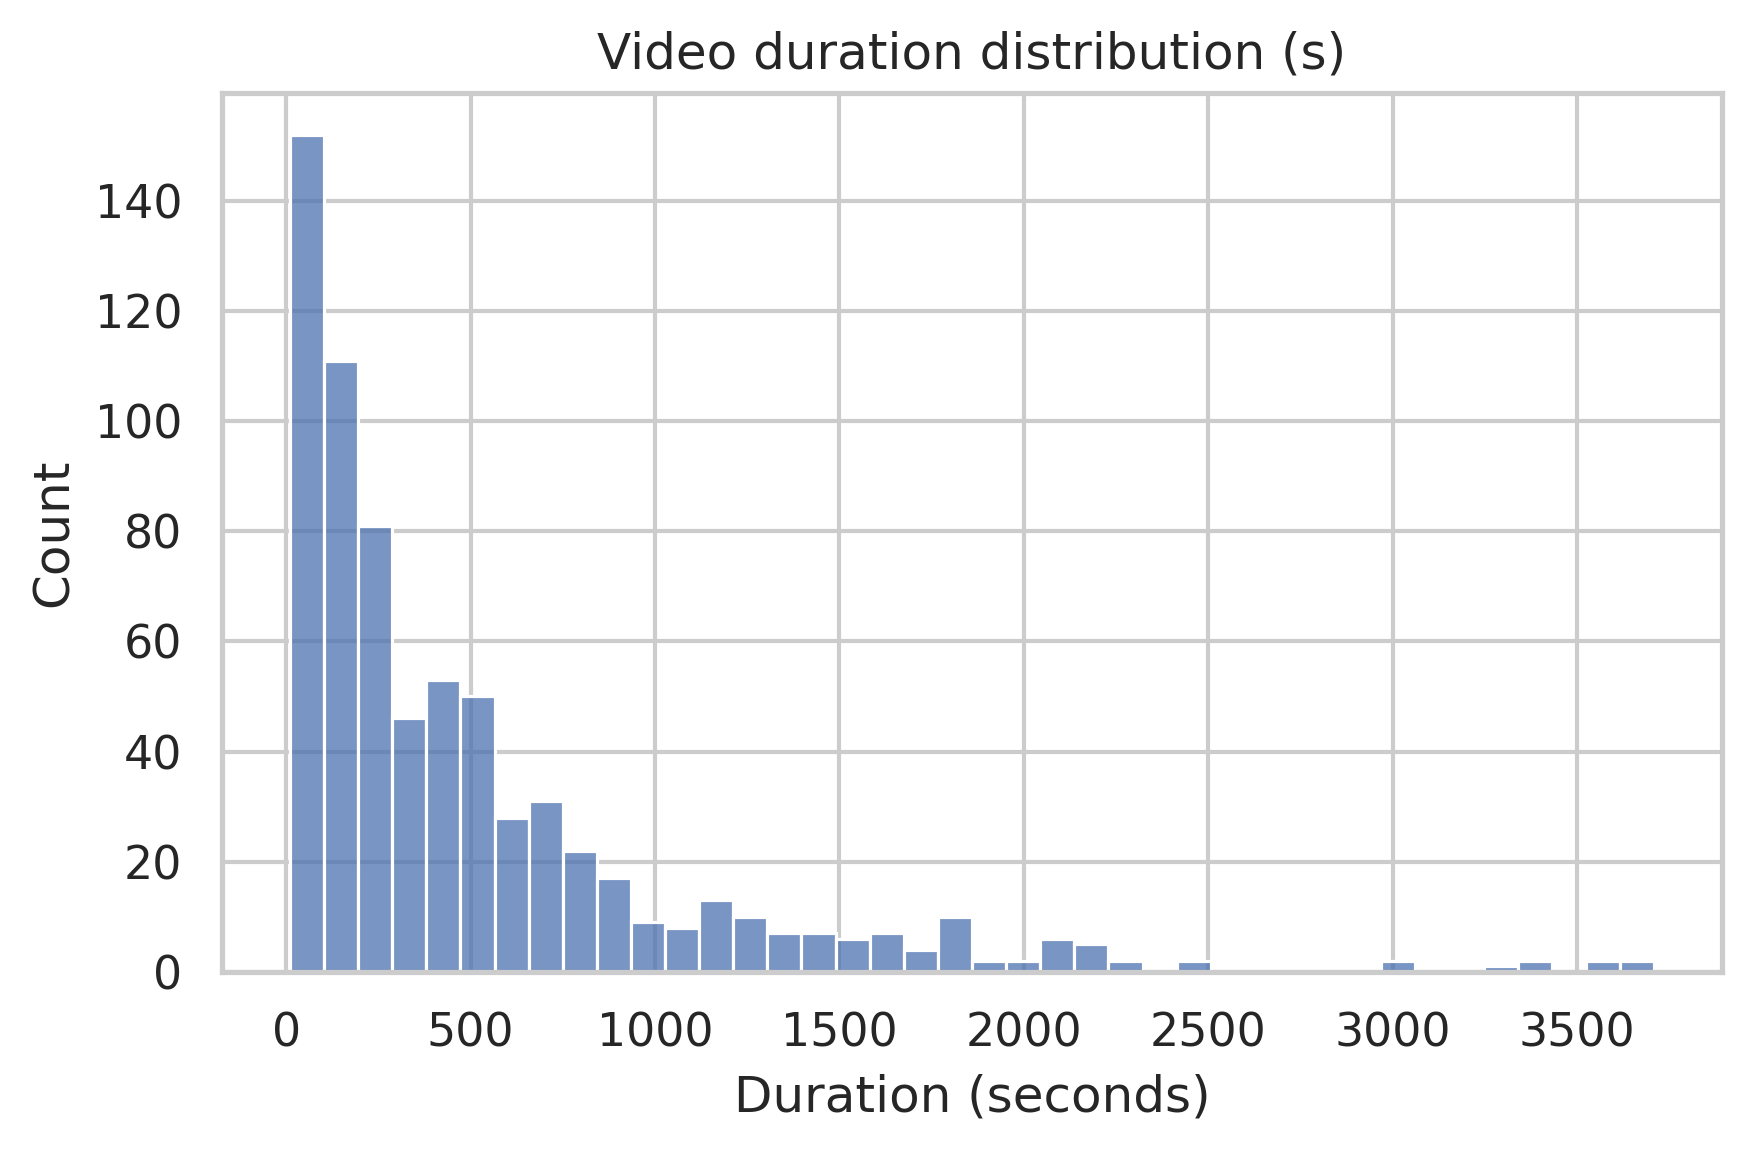
\includegraphics[width=\textwidth]{images/video_duration_hist.png}
        \caption{Video duration.}
        \label{fig:video_duration_hist}
    \end{subfigure}
    \hspace{0.01\textwidth}
    \begin{subfigure}[b]{0.31\textwidth}
        \centering
        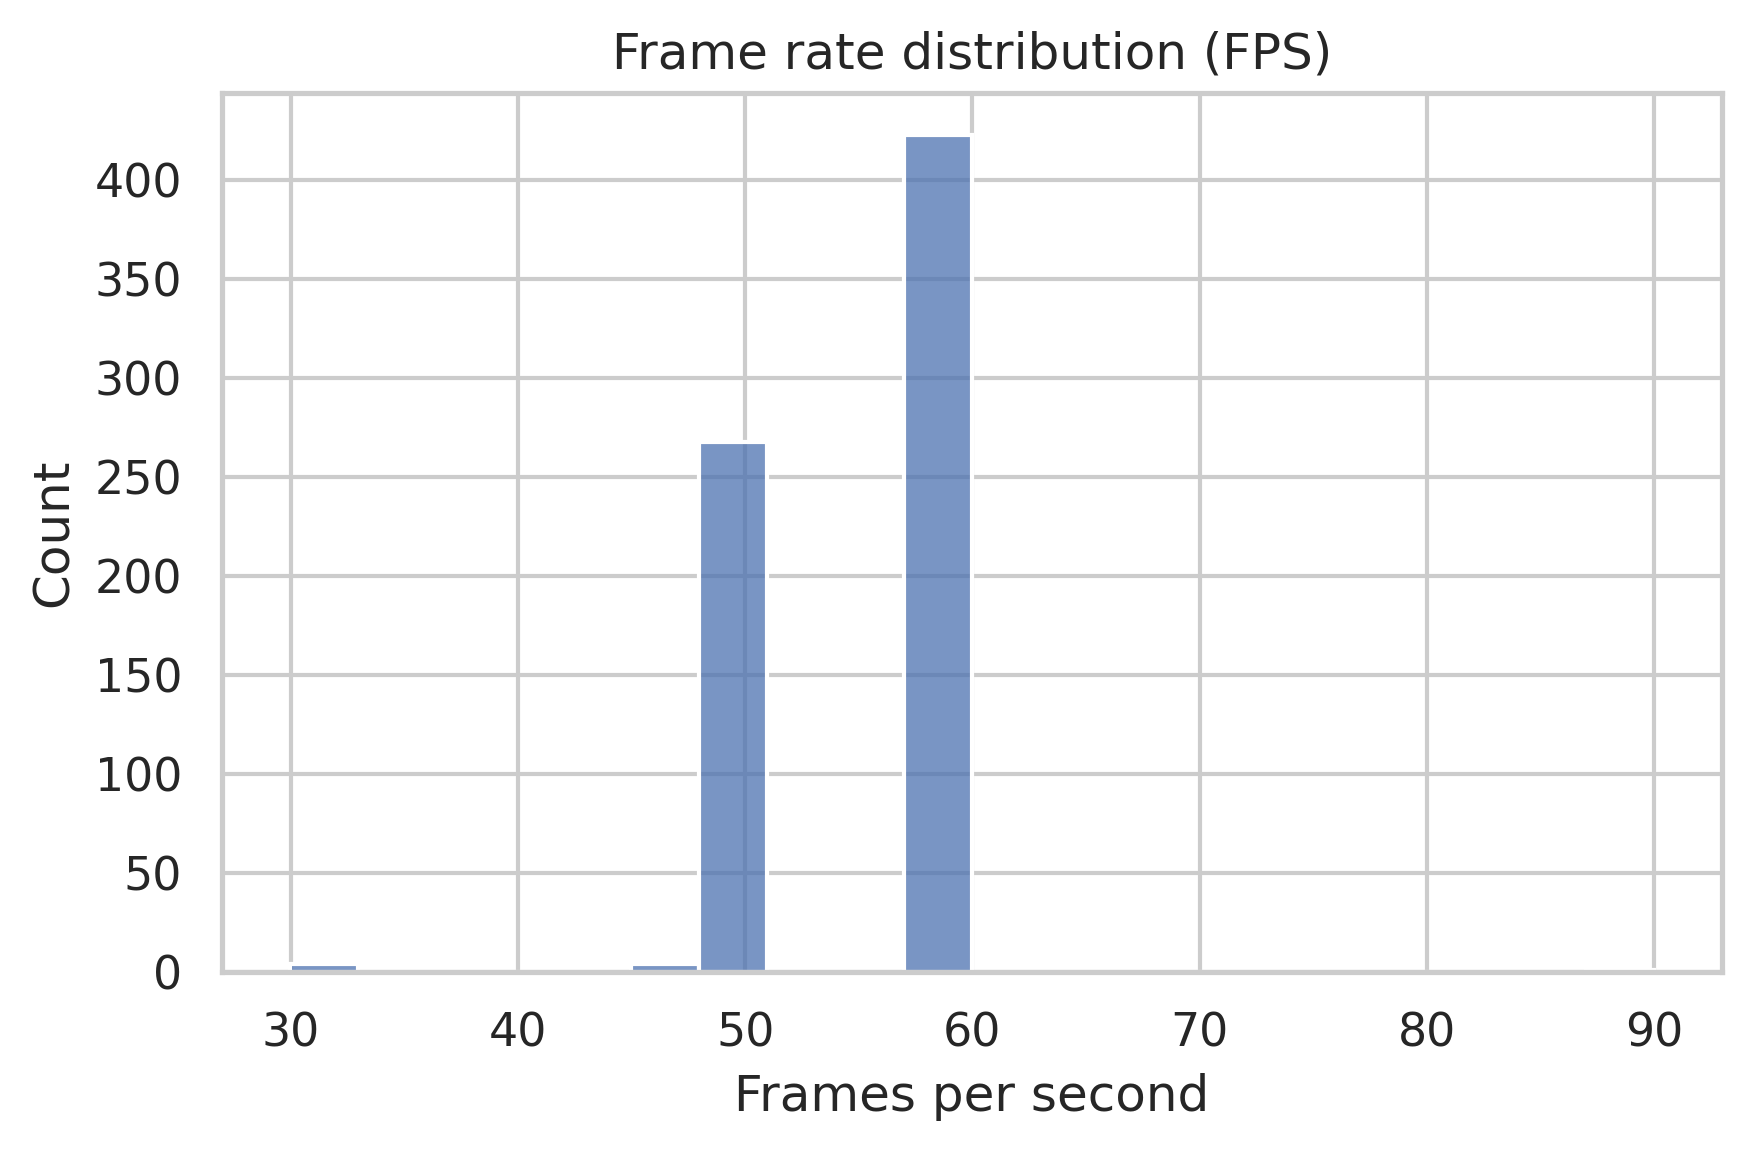
\includegraphics[width=\textwidth]{images/fps_hist.png}
        \caption{Frame rate.}
        \label{fig:fps_hist}
    \end{subfigure}
    \hspace{0.01\textwidth}
    \begin{subfigure}[b]{0.32\textwidth}
        \centering
        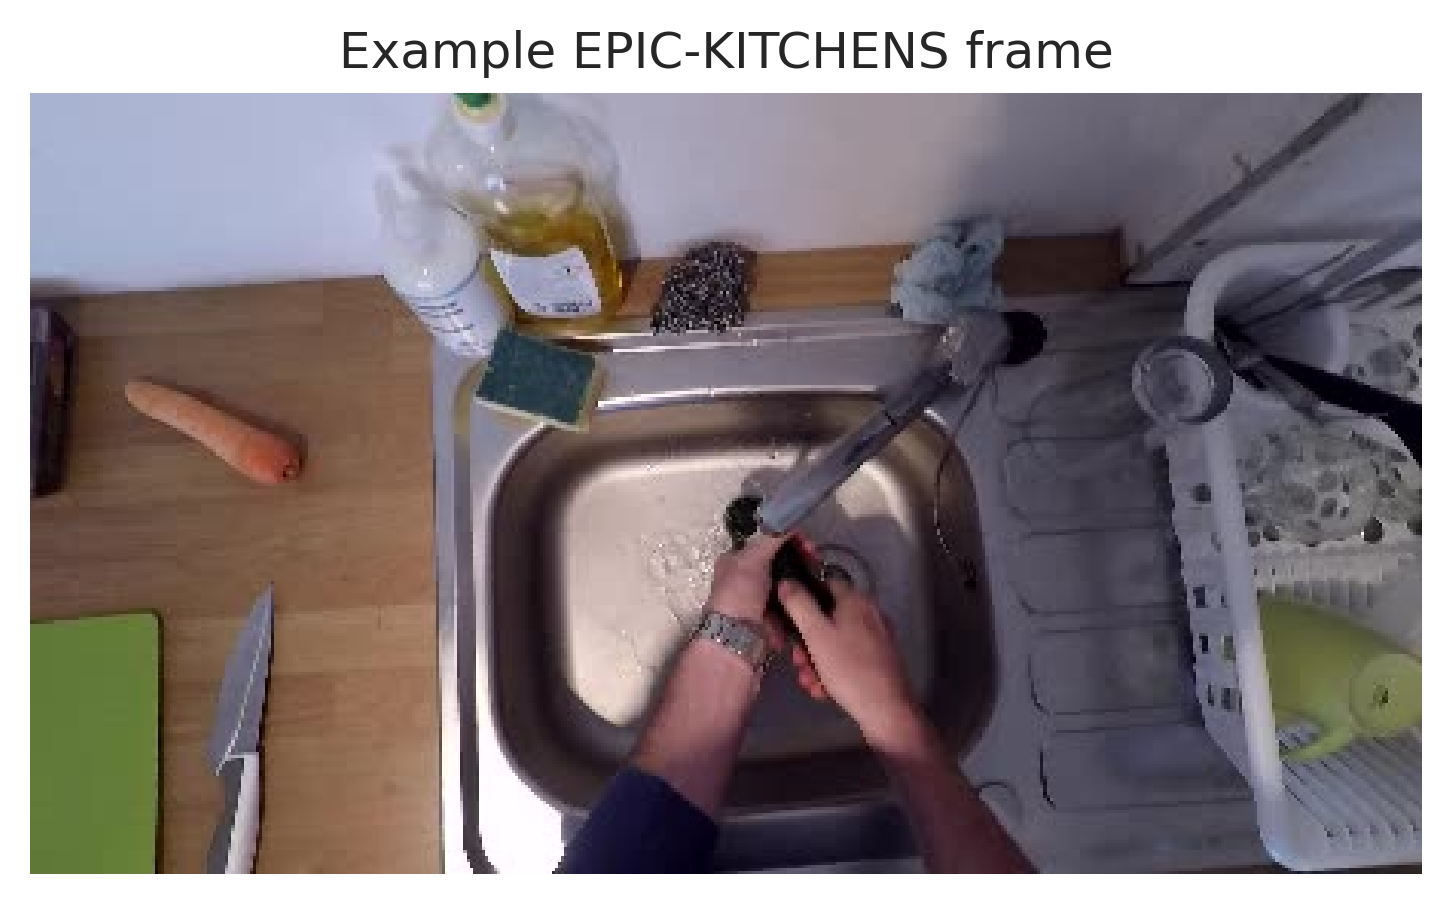
\includegraphics[width=\textwidth]{images/example_frame.png}
        \caption{Example frame.}
        \label{fig:example_frame}
    \end{subfigure}
    \caption{Video-level distributions of duration (s) and frame rate (fps) and a representative training frame illustrating the egocentric viewpoint and typical kitchen clutter.}
    \label{fig:video_stats}
\end{figure}

\paragraph{Segment-level statistics for MIR.}
Segment durations are computed from the retrieval annotation files as $\texttt{dur} = (\texttt{stop\_frame} - \texttt{start\_frame} + 1)/\texttt{fps}$. For the $67{,}217$ training segments, the mean is $3.18$\,s (std.\ $5.53$, median $1.6$, IQR $[1.0, 3.18]$\,s), confirming that most clips are very short while a long tail of extended actions reaches $\sim 297$\,s. This long tail motivates the choice of clip length used by our AVION-based fine-tuning pipeline (Section~\ref{sec:methods:avion}), where short default clips of 8 frames are augmented at test time to 32 frames for richer temporal context.

\subsection{Pre-trained checkpoints, hardware and software}
\label{sec:materials:stack}

Each approach reuses publicly released checkpoints. Approaches~1 and~2 operate on pre-extracted features and were executed on a single NVIDIA T4 (16\,GB) provided by Google Colab, using the JPoSE and MMEN encoders distributed by Wray et al.~\cite{wray2019jpose} together with the MI-MM checkpoint and S3D-HowTo100M features released alongside MIL-NCE~\cite{miech2020milnce}. Approach~3 fine-tunes a ViT-L/14 backbone from the AVION pre-train checkpoint of Zhao and Kr\"ahenb\"uhl~\cite{zhao2023avion}. It was deployed on a single NVIDIA A100 (40\,GB), with gradient checkpointing, the \texttt{use-fast-conv1} optimization of AVION and FlashAttention~\cite{dao2022flashattention} when available, halving attention memory at no accuracy cost, AdamW optimization ~\cite{loshchilov2019adamw}, a base learning rate of $2\times 10^{-5}$ and batch size $48$. Approach~3 also requires staging $\approx 720$\,GB of EK-100 video chunks (320p, 15\,s, 30\,fps, libx264) on persistent storage, together with the EK-100 retrieval annotations and the public training relevancy matrix~\cite{wray2021semantic}. As mentioned, the test relevancy matrix is held out by the organizers and not used at any stage. The implementation is built on PyTorch 2.4.1 (CUDA 12.1) with the standard vision--language components (\texttt{open\_clip\_torch}, \texttt{openai/CLIP}, \texttt{transformers}, \texttt{timm}), \texttt{decord} for video I/O, and \texttt{numpy}/\texttt{scipy.sparse} for the ensemble and re-ranking of Approach~2. Submissions are packaged as pickle protocol 2 with a numpy namespace compatibility shim required by the Codabench grader. The SMS-Loss code used in Approach~3 is a patched fork of the public release~\cite{wang2024smsloss_repo,wang2024symmetricmultisimilaritylossepickitchens100} that fixes a small number of bugs preventing stable end-to-end runs on EK-100 (tuple unpacking in the gradient-accumulation branch, an undefined \texttt{accum\_freq} reference replaced by \texttt{update\_freq}, dataloader retry logic for missing or corrupt video chunks, and \texttt{module.}-prefix stripping when loading \texttt{DataParallel}-wrapped checkpoints).


% Methods
\section{Methods}
\label{sec:methods}

We approached EK-100 MIR as an iterative search through the design space, starting from a feature-based zero-fine-tuning baseline and ending with end-to-end fine-tuning of a strong egocentric backbone with soft-label supervision. The three approaches share a common formalisation, stated once before each iteration is described.

\subsection{Task formalisation and common notation}
\label{sec:methods:formalisation}

Let $\mathcal{V} = \{v_i\}_{i=1}^{N_v}$ denote the $N_v = 9{,}668$ test video segments and $\mathcal{T} = \{t_j\}_{j=1}^{N_t}$ the $N_t = 3{,}842$ unique text queries on the test split. A retrieval system produces a similarity matrix $S \in \mathbb{R}^{N_v\times N_t}$ such that $S_{ij}$ is large when $v_i$ is semantically relevant to $t_j$. Ground-truth relevance is encoded in the soft-label matrix $R \in [0,1]^{N_v\times N_t}$~\cite{wray2021semantic}; the official challenge metric is the average normalised discounted cumulative gain
\begin{equation}
\mathrm{nDCG}_{\mathrm{AVG}} = \tfrac{1}{2}\bigl(\mathrm{nDCG}_{\mathrm{V\to T}}(S, R) + \mathrm{nDCG}_{\mathrm{T\to V}}(S^{\!\top}\!, R^{\!\top})\bigr),
\label{eq:ndcg}
\end{equation}
which captures both retrieval directions on equal footing. The three approaches differ only in how $S$ is constructed; the evaluation protocol is identical across them. Figure~\ref{fig:solutionflow} summarises the resulting pipeline.

\begin{figure}[t]
    \centering
    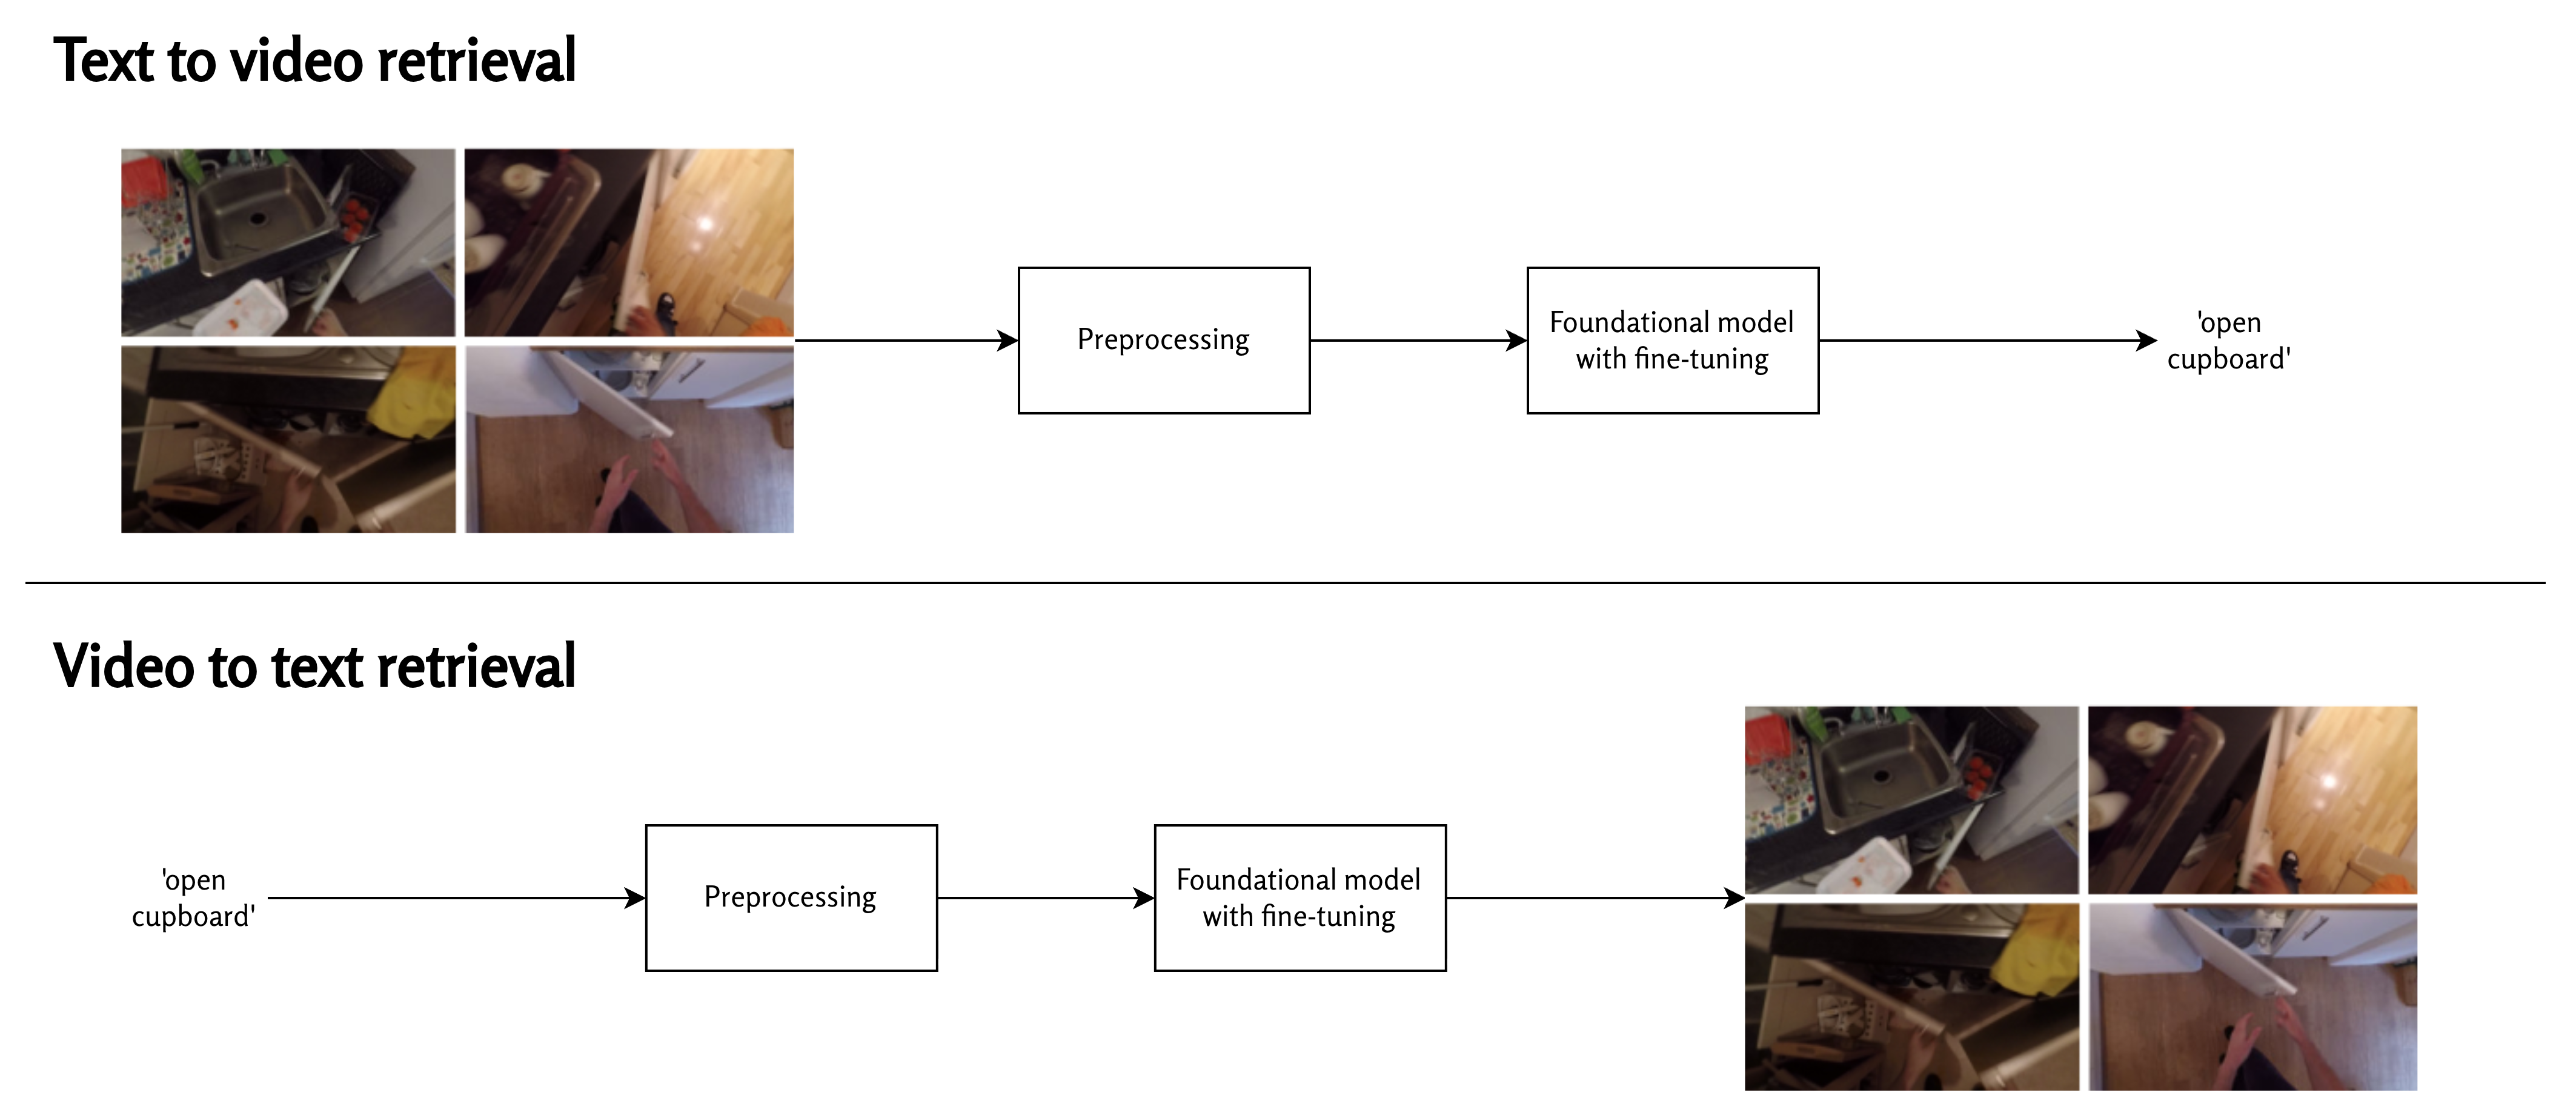
\includegraphics[width=0.7\textwidth]{images/flow.png}
    \caption{Overview of the multi-instance retrieval pipeline shared by the three approaches: visual and textual encoders project segments and queries into a shared space, and the resulting similarity matrix $S$ is ranked and evaluated against the soft-label matrix $R$. Image components adapted from~\cite{damen2022rescaling}.}
    \label{fig:solutionflow}
\end{figure}

\subsection{Approach 1: JPoSE Part-of-Speech baseline}
\label{sec:methods:jpose}

Our entry point is a feature-based, zero-fine-tuning baseline using JPoSE~\cite{wray2019jpose}, which projects segments and queries into three sub-spaces---verb, noun and full-action---learnt jointly with triplet supervision. Let $\phi^{\mathrm{v}}_{\mathrm{V}}, \phi^{\mathrm{v}}_{\mathrm{N}}, \phi^{\mathrm{v}}_{\mathrm{A}}$ and $\phi^{\mathrm{t}}_{\mathrm{V}}, \phi^{\mathrm{t}}_{\mathrm{N}}, \phi^{\mathrm{t}}_{\mathrm{A}}$ denote the visual and textual sub-encoders. We compute joint embeddings as the concatenation $\mathbf{f}_{\mathrm{v}}(v_i) = [\phi^{\mathrm{v}}_{\mathrm{V}}(v_i)\,;\,\phi^{\mathrm{v}}_{\mathrm{N}}(v_i)\,;\,\phi^{\mathrm{v}}_{\mathrm{A}}(v_i)]$ and analogously $\mathbf{f}_{\mathrm{t}}(t_j)$, and obtain $S^{\mathrm{JPoSE}}_{ij} = \cos(\mathbf{f}_{\mathrm{v}}(v_i), \mathbf{f}_{\mathrm{t}}(t_j))$. We use the released \texttt{JPoSE\_BEST} checkpoint without modification on pre-extracted features. By design this approach cannot exploit $R$ and inherits the limitations of triplet supervision with binary positives and negatives, but it provides a reproducible reference point against which all subsequent iterations are compared.

\subsection{Approach 2: score-level ensemble with graph-diffusion re-ranking}
\label{sec:methods:ensemble}

The second approach asks how far a purely inference-time strategy can carry the JPoSE baseline by combining several pre-trained retrieval models and refining the result with neighbourhood-aware re-ranking. Three complementary models are queried independently: $S^{\mathrm{JPoSE}}$ as in Section~\ref{sec:methods:jpose}; $S^{\mathrm{MI\text{-}MM}}$, the multi-instance MaxMargin model of Miech et al.~\cite{miech2020milnce} with S3D-HowTo100M features at the released best epoch (202); and $S^{\mathrm{MMEN}}$, an MLP-based Multi-Modal Embedding Network released as a baseline in~\cite{wray2019jpose}.

\paragraph{Step 1: row-wise normalisation and equal-weight fusion.}
The three matrices live on different scales (cosine similarities for JPoSE/MMEN, max-margin distances for MI-MM), so a direct sum is biased towards the highest-magnitude model. We min-max normalise each matrix \emph{row-wise} so that, for every video query, scores against the $3{,}842$ candidates are mapped to $[0,1]$:
\begin{equation}
\widetilde{S}^{(m)}_{ij} = \frac{S^{(m)}_{ij} - \min_k S^{(m)}_{ik}}{\max_k S^{(m)}_{ik} - \min_k S^{(m)}_{ik}}\,,\quad
S^{\mathrm{ens}} = \tfrac{1}{3}\,(\widetilde{S}^{\mathrm{JPoSE}} + \widetilde{S}^{\mathrm{MI\text{-}MM}} + \widetilde{S}^{\mathrm{MMEN}}).
\label{eq:ensemble}
\end{equation}
Equal weights are the natural default in the absence of a relevance-aligned validation signal.

\paragraph{Step 2: graph-diffusion re-ranking on visual and textual k-NN graphs.}
Inspired by diffusion-based re-ranking in image retrieval~\cite{iscen2017diffusion} and k-reciprocal encoding~\cite{zhong2017kreciprocal}, we propagate ensemble scores through the local geometry of the retrieval space in both modalities. After L2-normalising each row of $S^{\mathrm{ens}}$, a sparse visual affinity matrix $A_{\mathrm{vv}} \in \mathbb{R}^{N_v\times N_v}$ stores cosine similarity between the score profiles of each pair of segments if either is among the top-$k$ visual neighbours of the other; the same construction on $(S^{\mathrm{ens}})^{\!\top}$ yields a textual affinity $A_{\mathrm{tt}}$. We then expand the score matrix in both directions and blend with the original ensemble:
\begin{equation}
S^{\mathrm{exp}} = \tfrac{1}{2}\,(A_{\mathrm{vv}}\,S^{\mathrm{ens}} + (A_{\mathrm{tt}}\,(S^{\mathrm{ens}})^{\!\top})^{\!\top}),\quad
S^{\mathrm{rerank}} = (1-\alpha)\,S^{\mathrm{ens}} + \alpha\,S^{\mathrm{exp}},
\label{eq:rerank}
\end{equation}
with default $k=20$, $\alpha=0.3$. Both the ensemble matrix~\eqref{eq:ensemble} and the re-ranked matrix~\eqref{eq:rerank} are submitted to Codabench as separate iterations, isolating the contribution of re-ranking.

\subsection{Approach 3: AVION ViT-L fine-tuned with the SMS loss}
\label{sec:methods:avion}

The third approach replaces inference-time fusion with end-to-end fine-tuning of a strong CLIP-style egocentric backbone, supervised with the soft-label relevance matrix. The visual encoder is the AVION ViT-L/14 of Zhao and Kr\"ahenb\"uhl~\cite{zhao2023avion}, pre-trained on Ego4D via LaViLa~\cite{zhao2023lavila}; the textual encoder is the CLIP text transformer paired with that AVION checkpoint. Both encoders are fine-tuned jointly with the Symmetric Multi-Similarity loss of Wang, Wang and Chau~\cite{wang2024symmetricmultisimilaritylossepickitchens100}.

\paragraph{Symmetric Multi-Similarity loss.}
Within a training batch of $B$ video--text pairs, let $\mathbf{x}_i, \mathbf{y}_i \in \mathbb{R}^d$ denote the L2-normalised visual and textual embeddings of pair $i$, $r_{ij} \in [0,1]$ the soft relevance between $v_i$ and $t_j$ extracted from $R$~\cite{wray2021semantic}, and $s_{ij} = \mathbf{x}_i^{\!\top}\mathbf{y}_j$. The SMS loss extends the multi-similarity formulation of~\cite{wang2019multisimilarity} so that, instead of binary pair weights, the contribution of each pair is modulated by $r_{ij}$. With margin $\theta$, relevance threshold $\tau$ and temperatures $\beta_p, \beta_n$,
\begin{equation}
\mathcal{L}^{\mathrm{V\to T}}_i = \tfrac{1}{\beta_p}\log\!\Bigl(1 + \!\!\sum_{j: r_{ij}\ge \tau}\!\! r_{ij}\,e^{-\beta_p(s_{ij}-\theta)}\Bigr) + \tfrac{1}{\beta_n}\log\!\Bigl(1 + \!\!\sum_{j: r_{ij}<\tau}\!\! (1-r_{ij})\,e^{\beta_n(s_{ij}-\theta)}\Bigr),
\label{eq:sms}
\end{equation}
and the full loss is the symmetric counterpart $\mathcal{L} = \tfrac{1}{2}(\mathcal{L}^{\mathrm{V\to T}} + \mathcal{L}^{\mathrm{T\to V}})$ averaged over the batch. Compared with InfoNCE-like contrastive losses, SMS pulls together pairs in proportion to their relevance and pushes apart pairs in proportion to $1 - r_{ij}$, providing a supervision signal directly aligned with the nDCG metric.

\paragraph{Fine-tuning configuration.}
Fine-tuning is launched from the AVION pretrain checkpoint via \texttt{ammplus\_finetune.py} from a patched fork of the public SMS-Loss codebase~\cite{wang2024smsloss_repo} on a single A100. Key flags: \texttt{--model CLIP\_VITL14}, \texttt{--batch-size 48}, \texttt{--lr 2e-5}, \texttt{--loss-margin 0.6}, \texttt{--loss-thres 0.1}, with \texttt{--use-fast-conv1}, \texttt{--grad-checkpointing} (essential for ViT-L on a single GPU) and \texttt{--use-flash-attn} when available; FlashAttention~\cite{dao2022flashattention} roughly halves attention memory at no accuracy cost. Optimisation uses AdamW~\cite{loshchilov2019adamw}; one numbered checkpoint is saved per epoch. The relevance threshold $\tau = 0.1$ excludes pairs whose soft relevance is too small to provide a useful gradient and the margin $\theta = 0.6$ controls the separation enforced between positive and negative pairs; both values are inherited from the public reference configuration of~\cite{wang2024symmetricmultisimilaritylossepickitchens100}. A trained model can be extended at any point by passing both \texttt{--pretrain-model} and \texttt{--resume} pointing to the same checkpoint and increasing \texttt{--epochs}; we use this hook to extend the base 10-epoch run to 16 epochs.

\paragraph{Divergences from the published recipe.}
Two configuration choices depart from the SMS-Loss recipe of Wang et al.~\cite{wang2024symmetricmultisimilaritylossepickitchens100} and shape the upper bound of what our pipeline can achieve. First, our effective batch size of $48$ on a single A100 is approximately five times smaller than the $240$ samples (60 per GPU $\times$ 4 GPUs) reported for ViT-L by the original authors; smaller batches reduce the diversity of negatives visible to the SMS denominator in Eq.~\eqref{eq:sms} and weaken the metric-learning signal. Second, our base run is restricted to 10 epochs (extended to 16 in iteration~6) against the 100 epochs of the published recipe. Both deviations are quantified in Section~\ref{sec:conclusions:limitations} and motivate the future-work direction in Section~\ref{sec:conclusions:future}.

\paragraph{Inference and test-time augmentation.}
Inference is performed by \texttt{test\_mir.py}, which encodes all test video segments and text queries and writes a similarity matrix in the same format as Approaches~1 and~2. We compare two settings: a \emph{standard} pass with default 8-frame clips, and a \emph{TTA} pass with \texttt{--flip --clip-length 32} that averages the embeddings of the original and horizontally-flipped clips and samples 32 frames per segment. Flip-averaging is the canonical video adaptation of~\cite{krizhevsky2012alexnet} and exploits the near-invariance of kitchen activities to horizontal reflection; the longer clip length is motivated by the long tail of segment durations in Section~\ref{sec:materials:data}.


% Results
\section{Results}
\label{sec:results}

\subsection{Evaluation protocol}
\label{sec:results:protocol}

All configurations are evaluated under a single protocol on the official EPIC-KITCHENS-100 MIR benchmark on Codabench\footnote{\url{https://www.codabench.org/competitions/12008/}}. Each submission is a Codabench-compatible ZIP containing the $9{,}668\times 3{,}842$ similarity matrix serialized as a protocol-2 pickle with a numpy namespace shim. It is scored by the grader against the held-out test relevance matrix~\cite{wray2021semantic} and the grader returns the average nDCG (Eq.~\ref{eq:ndcg}) used to rank submissions. Because the test relevance matrix is not publicly released, mAP and per-direction nDCG cannot be computed offline; the official Codabench leaderboard nDCG~AVG is therefore the single primary metric.

\subsection{Comparative results across configurations}
\label{sec:results:main}

Table~\ref{tab:iterations} reports the official Codabench nDCG~AVG for each of the six submitted configurations described in Sections~\ref{sec:methods:jpose}--\ref{sec:methods:avion}, with the marginal change between consecutive submissions. The trajectory closes more than half of the gap between feature-based baselines and the current public state of the art (CR-CLIP at 82.10~nDCG~\cite{he2025crclip}) on a single GPU and using a total of sixteen epochs of fine-tuning.

\begin{table}[t]
\centering
\small
\caption{Official Codabench nDCG~AVG (\%) for the six submitted configurations of Section~\ref{sec:methods}. The $\Delta$ column reports the marginal change with respect to the previous row. Best per approach in \textbf{bold}.}
\label{tab:iterations}
\setlength{\tabcolsep}{6pt}
\resizebox{\textwidth}{!}{%
\begin{tabular}{l l l c c}
\toprule
\textbf{\#} & \textbf{Approach} & \textbf{Change w.r.t.\ previous row} & \textbf{nDCG AVG} & $\Delta$ \\
\midrule
1 & A1 -- JPoSE      & Feature-based baseline (no fine-tune)             & 53.53 & --     \\[1pt]
\midrule
2 & A2 -- Ensemble   & + 3-model ensemble (no re-ranking)                & 55.31 & +1.78  \\
3 & A2 -- Ensemble   & + Graph-diffusion re-ranking ($k{=}20$, $\alpha{=}0.3$) & \textbf{55.82} & +0.51  \\
\midrule
4 & A3 -- AVION+SMS  & Replace pipeline by AVION ViT-L + SMS, 10 ep      & 68.80 & +12.98 \\
5 & A3 -- AVION+SMS  & + TTA: \texttt{--flip --clip-length 32}           & 69.48 & +0.68  \\
6 & A3 -- AVION+SMS  & + 6 additional fine-tuning epochs (10 ep + 6 ep, 16 total) & \textbf{69.68} & +0.20  \\
\midrule
\multicolumn{3}{l}{\textit{Public leaderboard SOTA, CR-CLIP~\cite{he2025crclip}}}    & 82.10 & --     \\
\multicolumn{3}{l}{\textbf{Total improvement, configuration~1 $\to$ configuration~6}} & --   & \textbf{+16.15} \\
\bottomrule
\end{tabular}
}
\end{table}

The results show a clear hierarchy of effects. First, ensemble fusion of the three frozen pretrained models contributes $+1.78$~nDCG over the JPoSE baseline, indicating that JPoSE, MI-MM and MMEN are complementary enough for score averaging to recover variance that none of them captures individually. Second, graph-diffusion re-ranking adds $+0.51$~nDCG on top of the ensemble at no training cost, consistent with the magnitude of the gains reported in image retrieval~\cite{iscen2017diffusion}. Third, replacing the inference-time pipeline with the AVION ViT-L + SMS configuration produces the largest jump in the table, $+12.98$~nDCG. Fourth, post-fine-tuning refinements behave as expected: TTA adds $+0.68$~nDCG at no training cost, and continuing fine-tuning for six additional epochs on top of the initial 10-epoch run (16 epochs in total) adds $+0.20$~nDCG, suggesting that single-checkpoint training is approaching its plateau.


% Discussion
\section{Discussion}
\label{sec:discussion}

The per-configuration breakdown in Table~\ref{tab:iterations} concentrates 80\% of the total improvement (12.98 of 16.15 nDCG points) in the single transition from Approach~2 to Approach~3. That is from a frozen-feature ensemble to an end-to-end fine-tuned ViT-L driven by soft-label supervision. The asymmetry across the configurations is itself the central observation, and it can be unpacked along three connected lines: the low ceiling of inference-time refinements over frozen backbones, the dominant effect of the bundled encoder-and-loss swap, and the diminishing returns of post-fine-tuning refinements that motivate the future-work direction.

Approach~2 fuses three pre-trained models that were never optimized for the soft-label setting: JPoSE and MMEN are triplet-supervised, MI-MM is binary multi-instance MaxMargin, and none sees the relevance matrix $R$ during training. Equal-weight averaging of their normalized scores recovers $+1.78$~nDCG on top of JPoSE, in line with the canonical observation that retrieval ensembles reduce variance without correcting bias~\cite{wortsman2022modelsoups}. Because the three models share the same failure mode (they ignore graded relevance), averaging them produces a more stable estimate of the same flawed objective rather than one that is closer to nDCG. Equal weights were used in the absence of a relevance-aligned validation signal and weighted averaging tuned on a held-out split could plausibly add a fraction of a point but is unlikely to overcome the bias ceiling. Graph-diffusion re-ranking adds another $+0.51$~nDCG at no training cost, consistent with magnitudes reported for diffusion in image retrieval~\cite{iscen2017diffusion}. A small $k=20$ keeps the affinity graph sparse and avoids over-smoothing, moderate $\alpha=0.3$ blends rather than replaces the original signal, and the symmetric construction in Eq.~\eqref{eq:rerank}---propagating through both visual and textual graphs---prevents either modality from dominating the result.

The single largest jump, $+12.98$~nDCG between configurations~3 and~4, is associated with a \emph{bundle of changes} introduced together at that step: pre-extracted features are replaced by an end-to-end ViT-L/14 encoder pre-trained on egocentric video~\cite{zhao2023avion,zhao2023lavila}, binary triplet/MaxMargin objectives are replaced by the SMS loss~\cite{wang2024symmetricmultisimilaritylossepickitchens100} that consumes the soft-label matrix $R$ directly, and both encoders are jointly fine-tuned rather than frozen. Because these changes were applied jointly and not ablated, we report the gain as a property of the bundle rather than attributing it causally to any single factor; disentangling the relative contribution of each ingredient would require an ablation study that was beyond our compute budget. What can be stated empirically is that the bundle dominates every other change in the table by an order of magnitude, and that the only mechanism in this bundle that directly optimises the nDCG metric (Eq.~\eqref{eq:ndcg}) is the SMS loss in Eq.~\eqref{eq:sms}, which weights both positive and negative pairs by their soft relevance. The size of the joint gain is consistent with the observation in~\cite{wray2021semantic} that graded-relevance objectives can reshape retrieval orderings well beyond what binary contrastive losses achieve.

Once the encoder has been fine-tuned end-to-end with SMS, however, further gains diminish quickly. TTA (\texttt{--flip --clip-length 32}) yields $+0.68$~nDCG with no training cost. Flip-averaging adapts the canonical recipe of~\cite{krizhevsky2012alexnet} to video and exploits the near-symmetry of kitchen scenes under horizontal reflection, while the longer clip length addresses the long tail of segment durations identified in Section~\ref{sec:materials:data}. Extending fine-tuning with six additional epochs on top of the initial 10-epoch run (16 epochs in total) adds a further $+0.20$~nDCG, suggesting the model is approaching the plateau of single-checkpoint training. This corresponds precisely to the regime in which model-averaging strategies tend to be most cost-effective and which motivates the future-work direction in Section~\ref{sec:future}. The practical implication of Table~\ref{tab:iterations} is that, under a tight compute budget, the bundle of encoder fine-tuning with relevance-aware supervision concentrates the bulk of the achievable improvement, while re-ranking and TTA are essentially free and should be applied by default, ensemble fusion of frozen baselines is also cheap but quickly hits a ceiling, and longer training is subject to rapidly diminishing returns. This ordering is consistent with what both the SMS-Loss authors~\cite{wang2024symmetricmultisimilaritylossepickitchens100} and the CR-CLIP authors~\cite{he2025crclip} report on the same benchmark, where most of the gap to the leaderboard is closed by the encoder and relevance-aware loss and subsequent refinements account for a smaller residual.


% Conclusions
\section{Conclusions}
\label{sec:conclusions}

We reported a controlled, empirical exploration of the EPIC-KITCHENS-100 Multi-Instance Retrieval challenge in which three configurations of increasing strength were evaluated under a single Codabench protocol. Starting from a JPoSE feature-based baseline at $53.53$\,nDCG, a score-level ensemble of three frozen retrieval models combined with graph-diffusion re-ranking lifts performance to $55.82$\,nDCG, while an AVION ViT-L/14 dual encoder fine-tuned with the SMS loss and complemented by horizontal-flip plus 32-frame test-time augmentation reaches $69.68$\,nDCG over sixteen epochs of single-GPU training. The strongest configuration recovers more than half of the gap between feature-based baselines and the current public state of the art (CR-CLIP, $82.10$\,nDCG~\cite{he2025crclip}) using a single A100 instance and the publicly released SMS-Loss training code. Since the transition between the second and third approach changes the encoder, the loss and the training regime jointly rather than in isolation, the per-row deltas in Table~\ref{tab:iterations} should be read as marginal effects of a configuration change rather than as a causal attribution. Subject to that caveat, the breakdown indicates that the bundle of end-to-end fine-tuning with a relevance-aware loss concentrates the bulk of the achievable improvement on a single GPU, while inference-time strategies contribute small but reliable deltas at zero training cost---providing a practical compute-allocation reference for future EK-100 MIR work operating under similar resource constraints.

\section{Limitations and Future Work}
\label{sec:limitations}

\subsection{Limitations}

Two limitations frame our results. First, all Approach~3 experiments were performed on a single NVIDIA A100 (40\,GB) with a batch size of $48$, which made multi-GPU runs, larger effective batch sizes and multi-seed re-training infeasible within the project timeline. Several knobs that are routine in the EK-100 MIR literature were therefore left unexplored. These include the contribution of larger batches (which directly affects the SMS gradient through the implicit hard-negative mining in Eq.~\eqref{eq:sms}), systematic sweeps over $\theta$, $\tau$, $\beta_p, \beta_n$, longer fine-tuning schedules above 16 epochs, and variance estimation through repeated runs with different random seeds. As a consequence, the bundled $+12.98$\,nDCG between Configuration~3 and Configuration~4 cannot be ablated into the individual contributions of encoder, loss and end-to-end training within this study. Second, the EK-100 challenge releases the soft-label relevance matrix only for the training split; the test relevance matrix required to compute nDCG and mAP offline is held out by the organizers and accessible exclusively through the Codabench grader. Model selection during fine-tuning therefore had to rely on training-loss trajectories rather than on a relevance-aligned validation signal, and every reported number in Table~\ref{tab:iterations} required a Codabench submission, which capped the practical iteration budget.

\subsection{Future work}
\label{sec:future}

The most promising extension consistent both with the empirical evidence in Table~\ref{tab:iterations} and with the SMS-Loss recipe of Wang et al.~\cite{wang2024symmetricmultisimilaritylossepickitchens100} is the \emph{score-level ensemble of multiple SMS-supervised checkpoints} described in Section~3.3 of that paper, which we did not have the compute budget to reproduce. Concretely, the published recipe combines six independent models: three Adaptive MI-MM variants with different learning-rate schedules and three SMS variants with different relaxation thresholds ($\tau \in \{0.05, 0.10, 0.12\}$). All six are trained for $100$ epochs from the same AVION pretrain~\cite{zhao2023avion} and are combined by directly summing their test similarity matrices, achieving an additional $+1.1$\,mAP and $+0.6$\,nDCG over the best single model. Replicating this ensemble on top of our AVION+SMS pipeline is a natural and well-defined extension: the row-wise normalization and equal-weight averaging of Approach~2 (Eq.~\eqref{eq:ensemble}) provide a drop-in replacement for the direct sum, and the graph-diffusion re-ranking of Eq.~\eqref{eq:rerank} can be stacked on top at no training cost. The rationale is supported by three observations from our trajectory and the related literature. First, longer training of a single ViT-L instance yields rapidly diminishing returns past 10--16 epochs, so additional compute is better invested in a few short complementary models than in extending a single one indefinitely. Second, model-soup-style strategies---in which several models fine-tuned with different hyperparameters but the same initialization are combined---consistently match or exceed the best individual model in image classification~\cite{wortsman2022modelsoups} and have already been shown to work in this exact retrieval setting~\cite{wang2024symmetricmultisimilaritylossepickitchens100}. Third, Approach~2 already validates the inference-time fusion machinery on weak frozen baselines, so deploying it on stronger fine-tuned ViT-L+SMS instances is essentially mechanical. The principal obstacle is computational: training six ViT-L+SMS instances for $100$ epochs each requires roughly $40\times$ the GPU-hours of our Configuration~6 and is not feasible on a single GPU within a typical project timeline. We therefore frame this direction as the natural continuation of the present work, conditional on multi-GPU infrastructure, in line with the $4\times 4$ RTX~6000~Ada configuration used by Wang et al.~\cite{wang2024symmetricmultisimilaritylossepickitchens100} for ViT-B and the 48\,GB GPUs used for ViT-L. Beyond the ensemble direction, two further extensions follow from the limitations above: integrating the context-refinement mechanism of CR-CLIP~\cite{he2025crclip} on top of our AVION+SMS pipeline (closing a documented portion of the gap to the public leaderboard), and replacing the SMS loss in Eq.~\eqref{eq:sms} with a directly differentiable nDCG surrogate adapted to graded relevance (Smooth-AP~\cite{brown2020smoothap} or a SoDeep-style ranker~\cite{engilberge2019sodeep}).



\bibliographystyle{splncs04}
\bibliography{bibliography}

\end{document}
